\section{Reinforcement Learning implementation}
\label{ch1:sec:reinforcement}

Two components support the Reinforcement Learning: the environment and the zone agent. 
The first one relates to a distribution network and its elements, whereas the second 
one to a learning agent.

The distribution network is susceptible to failures and switching operations, which modifies 
its topology and operation values. 
On the other hand, the zone agent performs Service Restoration on the environment to learn 
the optimal sequence of switching operations after a failure occurrence. 

Figure \ref{ch1:fig:mdp_blocks} presents the interaction between these two elements, which 
allows the algorithm to learn and to automate the decision-making process. This interaction 
is defined in the next section using a finite Markov Decision Process (MDP).

\begin{figure}
    \centering
    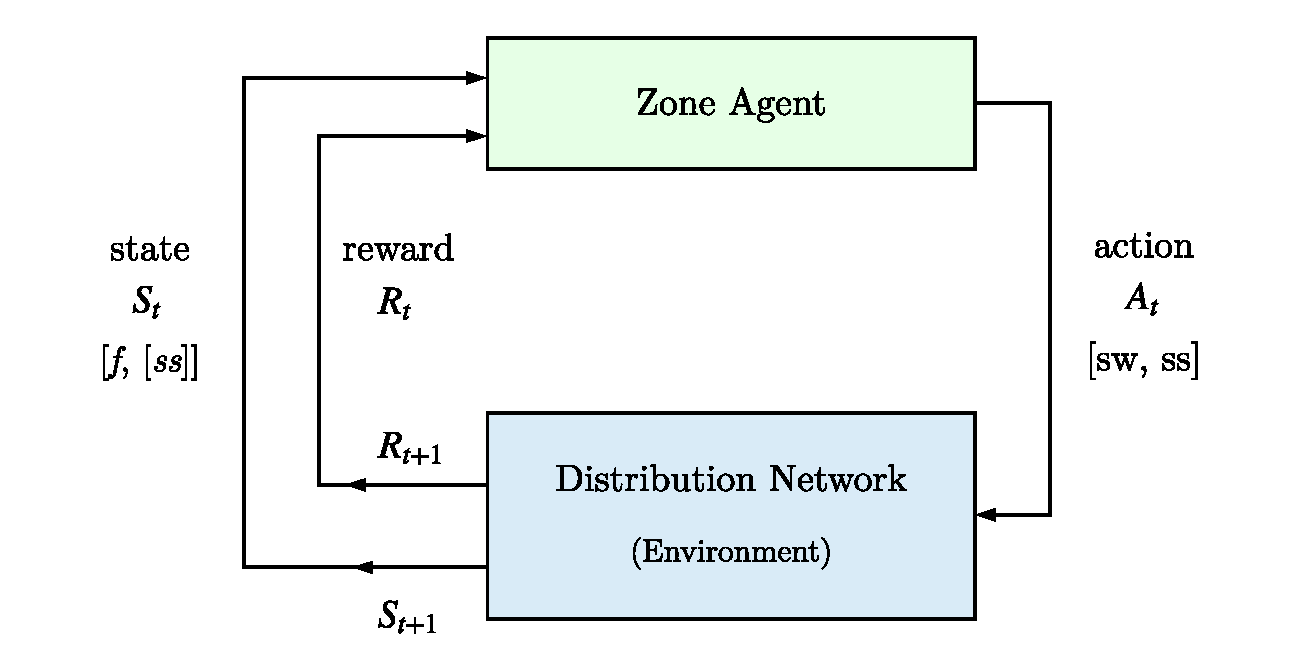
\includegraphics[scale=0.6]{_chapter1/fig/mdp_blocks}
    \caption{MDP block diagram}
    \label{ch1:fig:mdp_blocks}
\end{figure}

\subsection{Markov Decision Process}

MDP is a framework that defines the interaction between the agent and the environment in terms of states,
actions, and rewards. These terms are defined as follows:

\nomenclature[G]{MDP}{Markov Decision Process}

\subsubsection{MDP Elements}

A \textit{state} ($s_t$) defines how the environment is at a particular time and corresponds to an
ordered pair of two elements $[f, [ss]]$. The first element corresponds to a specific failure 
(\textit{f}), while the second one is an ordered list of zeros and ones representing the state of 
switches ($[ss]$). A closed switch takes the value of one, while an open switch takes zero.

Equation \ref{ch1:equ:num_states} returns the total number of states $n(S)$, from the numbers of switch 
status $n(ST)$, switches $n(SW)$, and lines $n(LN)$. 
\begin{equation}
\begin{split}
n(S) &= n(ST)^{n(SW)}*n(LN)\\
\end{split}
\label{ch1:equ:num_states}
\end{equation}

\nomenclature[H]{$n(S)$}{The number of states }
\nomenclature[H]{$n(ST)$}{The number of switch status}
\nomenclature[H]{$n(SW)$}{The number of switches}
\nomenclature[H]{$n(LN)$}{The number of lines}


\nomenclature[H]{$s_t$}{State at time step \textit{t}}
\nomenclature[H]{$[f, [ss]]$}{State: ordered pair of failure and the state of switches}
\nomenclature[H]{\textit{f}}{Failure}
\nomenclature[H]{\textit{$[ss]$}}{The state of switches (ordered list)}

An \textit{action} ($a_t$) is a selection, made by the agent, of which switch operates next. 
However, it does not define the switching operation. The decision if the selected switch opens or 
closes is determined by the opposite of its status, i.e., the agent chooses a switch instead of a 
switching operation. 

\nomenclature[H]{$a_t$}{Action taken at time step \textit{t}}

A \textit{policy} ($\pi$) tells the agent how to take actions from states. It can be 
deterministic or stochastic. 

\nomenclature[H]{$\pi$}{Policy of the Reinforcement Learning algorithm}

A \textit{reward signal} is a numeric value that rates a chosen action, from a given state, 
based on the Service Restoration constraints, e.g., it assigns a negative number for every 
violated restriction.

\subsubsection{MDP Interaction}

\begin{figure}
    \centering
    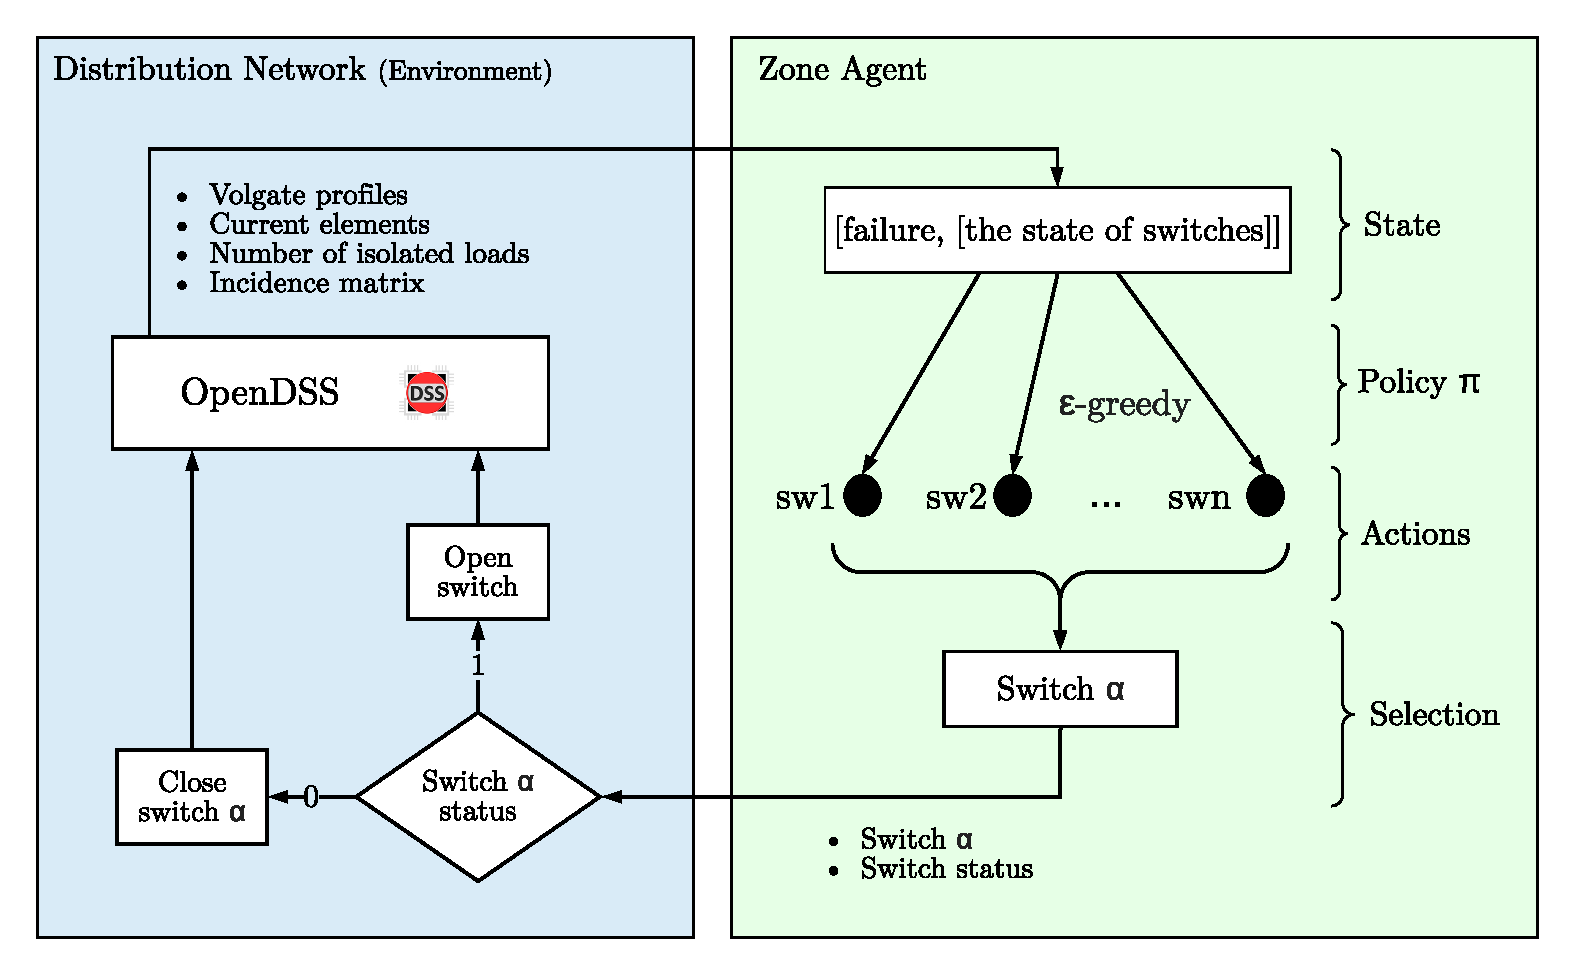
\includegraphics{_chapter1/fig/mdp_blocks_details}
    \caption{MDP block diagram details}
    \label{ch1:fig:mdp_blocks_details}
\end{figure}

A failure occurrence $f$ triggers the interaction between the environment and the agent.
The first to initialize is the environment. It gets its current state $[f,[ss]]$ and sends it to the 
zone agent, who uses it to know which are the possible actions from that state.
Secondly, the zone agent starts and chooses its first switch based on the $\epsilon$-greedy policy.
And then, it sends the switch to the environment, which checks its status and performs the 
corresponding switching operation. 

After the switching operation, the distribution network reaches the next state, which 
drives to new network parameters. These parameters include voltage and current profiles, 
number of isolated loads, and topology. Consequently, the environment compares them 
with the system constraints to verify their fulfillment and, relying on this, rewards 
the state-action pair. 

The reward depends on the number of violated constraints and their hierarchy. For this 
reason, the number of loads isolated receives the highest penalty, followed by voltage and 
current limits, and, lastly, the number of loops within the DN. 

To end the first interaction, the agent gets the reward and the next state and uses them 
to update the value of the previous state-switch pair. The switch-value update depends on 
the RL algorithm implemented. The present study implements two  RL algorithms, which are 
explained in the following section. 

After the action-value update, a new interaction begins, as described above, until the agent 
reaches the terminal state.  As a result, this performs an RL episode. But the agent needs 
hundreds of episodes to learn an optimal policy. 

Figure \ref{ch1:fig:mdp_blocks_details} summarized the details for the proposed MDP.



\subsection{RL episode}
\begin{figure}[!ht]
    \centering
    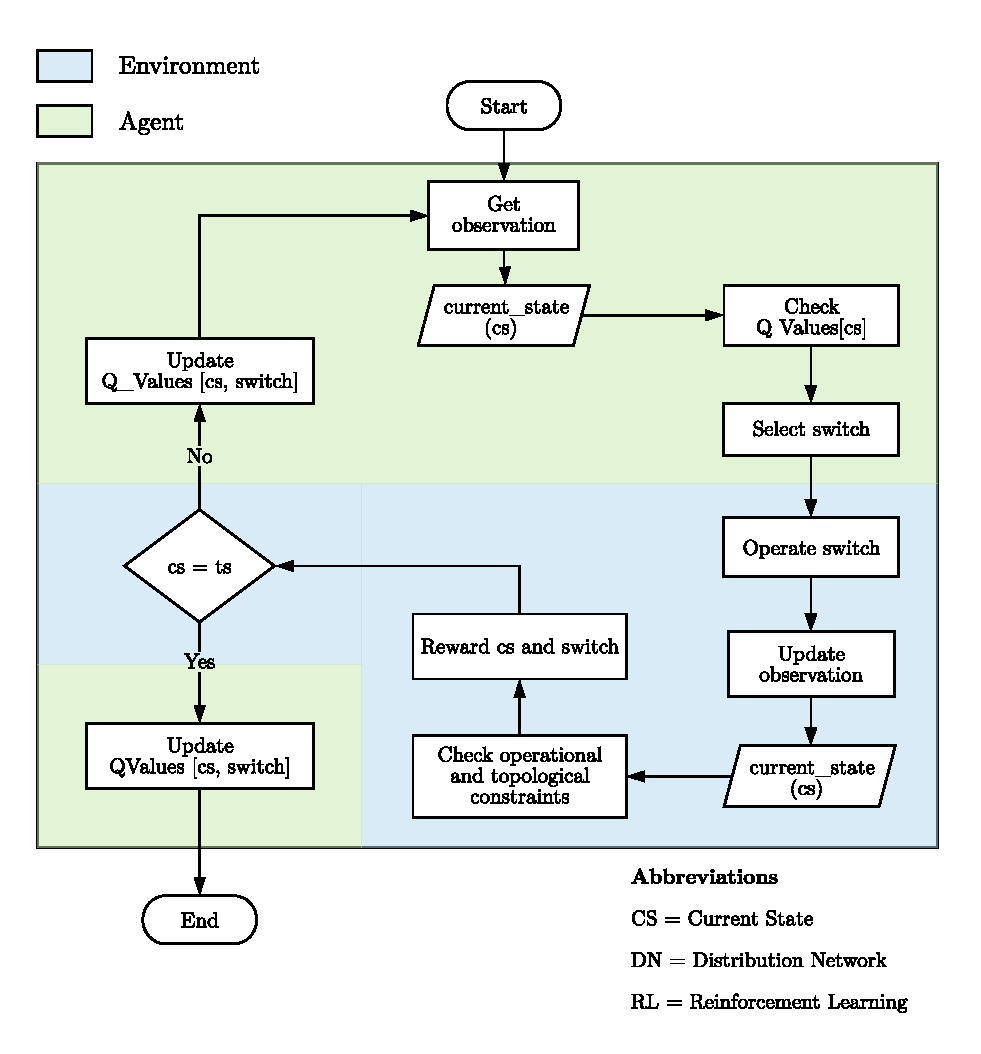
\includegraphics[scale=0.7]{_chapter1/fig/rl_episodes.pdf}
    \caption{Reinforcement Learning Episode}
    \label{ch1:fig:rl_episode_blocks}
\end{figure}

The previous section explains the detail of the MDP interaction between the environment and the agent. Each of those interactions corresponds to an episode. 

Figure \ref{ch1:fig:rl_episode_blocks} shows a block diagram for interaction, but this time from the Service Restoration algorithm perspective. 

%% AP ends ---------------------------

%The interaction starts with the environment initialization which includes a failure occurrence. The environment
%gets its current state $[f, [ss]]$ and sends it to the zone agent, who uses that information to choose a switch. 
%The switch is selected based on an e-greedy policy. The switch selected is sent to the environment, where it performs the switching operation, the switching operation is the opposite of the switch status. Then it collects information about the distribution network, which includes voltage and current profiles, number of isolated loads, and topology.  This data is used to rewards that action. 
%The reward is now sent to the agent with the new current state. The agent updates the value function and takes 
%the next switch. 


%\subsection{Q-learning}

%\subsubsection{Algorithm parameters}

%\subsection{Dyna-Q+}

%\subsubsection{Algorithm parameters}
%A \textit{policy} ($\pi$) says the agent how to take actions from states. The policy also differs from training and 
%production scenarios. The training policy is e-greedy which means that the actions are taken greedy
%1-e percert of the time. While the remaining e percent of the time, the actions are taken ramdonly. 
%This allows the agent to a continuos learning due to the agent explotes when the an action is taken 
%greedy and explore when the action is taken ramdonly. This is valid for training escenario but production 
%scenario, 
% not sure if the policy changes from scenarios 

%A \textit{reward signal} is an immediate sense of how good is the action taken, it takes into account the constrains 
%of the Service Restoration problem. And it assigns a value for every violated restriction. it helps to 
%define the goal of RL. The reward scheme is as follows: 

%Input data 
%In addition to the state, the environment gives the zone agent a package of information about the
%distribution network that includes voltages and currents profiles, number of isolated loads, and
%network topology. 


% que se hace si el espacio de actions y estado no es pequeño, no se puede usar un metodo tabular? 